\chapter{User interface design}
\label{chap:user_interface_design}
\section{Method}
\label{sec:method}
We have chosen several different methods and processes that enable us to achieve results in a consistent manner. In this section, we will describe the methods we have applied, and explain why they were chosen over similar alternatives.

\subsection{Iterative design}
When designing a user interface with the intention of reaching a high level of usability, a systematic approach is key. The process we have used, can be roughly divided in to 4 steps, where the latter part can be repeated until the Quality Requirements, listed in \ref{subsec:quality_requirements}, have been met. \cite{lauesen} \\
The steps are:
\begin{enumerate}
\item Analysis of users and tasks
\item Construct prototype
\item Perform usability tests
\item Amend prototype 
\end{enumerate}

The semester planning and day to day booking have been described seperately, due to the differences between them. We will provide a detailed walkthrough of the process for an element in each part, and the full history of mockups can be found in appendix \ref{app:mockups}.

\subsection{Usability testing}
\label{sec:usability_testing}
With usability being our primary focus, choosing a proper method of testing said usability is key. A number of different variations of user-based testing exist:\cite{lauesen}
\begin{itemize}
\item \textbf{Observe only} - Let the user work out the task on his own, and simply observe his struggles
\item \textbf{Think aloud} - Let the users explain their thoughts and decision as they (try to) complete the tasks
\item \textbf{Cooperation} - Have two users solve the tasks together, and encourage them to discuss what is going on
\end{itemize}

Among the most widely used technique for testing user interfaces in development stages are the think aloud method.\cite{steve} As one can imagine, not all test subjects find it natural to explain their thoughts as they go, but with interested questions from the test evaluator, most users get familiar with the concept very fast. We have chosen the think aloud test for two primary reasons.
First, because even in the worst cases where a user does not adapt to explaining why and what they do, you can still get the same, if not better, results than with the \emph{observe only} test.
Secondly, the \emph{cooperation} test has the potential danger of concealing usability problems. In the case where test subjects \emph{t1} and \emph{t2} are cooperating on a task, a problem t1 would have encountered alone, will not be discovered due to p2 solving it beforehand, and vice versa. This results in potentially only finding problems which both users would have encountered on their own.

Surprisingly, we have not found any description of this problem by the established experts, and can therefore not verify our theory, but have nonetheless decided to avoid this version of usability testing, based on this. \\
\\
Choosing which, and how many, test subjects is needed for a test is a heavily debated subject in the usability community. Most tend to agree that 5 or below is more than enough for each round. The controversy arise when figuring out how representative the test subjects most be for your target audience. Soren Lauesen opens the corresponding chapter with: \cite{lauesen}
\begin{quotation}
\noindent \emph{``A usability test must of course be made with users that correspond to the real users we expect in practice.''}
\end{quotation}
However, Steve Krug has a different view: \cite{steve}
\begin{quotation}
\noindent \emph{``The importance of recruiting representative users is overrated. [...]''} \\
\noindent \emph{``The best-kept secret of usability testing is the extent to which it doesn't much matter who you test.''}
\end{quotation}

What we can take away from their different arguments for and against, is that testing with representative users is \emph{good}, but not vital when it simply comes to eliminating problems.
We have chosen to do both. The system is intended to be used by everyone at ITU, which will also include newly started students and faculty.
Another point of agreement among the experts, is that testing early and often will \emph{always} trump testing with many users at a later point. \cite{lauesen,steve,nielsen_five_users}

The table in figure \ref{fig:usa_users} shows how many users have been tested for each part of the system for each round. As seen, we've opted to only test one user for the semester planning, which is simply due to the lack of people with the required knowledge, and the very narrow target audience.

\begin{figure}[htb]
\begin{center}
\leavevmode
	\begin{tabular}{|l|r|r|r||r|}
		\hline
		 & Round 1 & Round 2 & Round 3 & Total \\ \hline
		Day to day & 2 & 2 & 2 & 6\\ \hline
		Semester & 1 & 1 & n/a & 2 \\ \hline
	\end{tabular}
\end{center}
\caption{Overview of test users per round}
\label{fig:usa_users}
\end{figure}

\begin{figure}[htb]
\begin{center}
\leavevmode
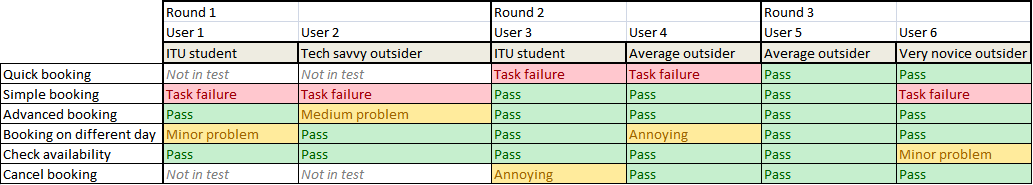
\includegraphics[width=1\textwidth]{images/result_day}
\end{center}
\caption{Test results for the day to day booking}
\label{fig:results_day}
\end{figure}

Figure \ref{fig:results_day} provides a full overview of our findings from the usability testing of the day to day system, which we will use as a reference in the day to day booking chapters. We have used the problem classification defined by Soren Lauesen\cite{lauesen}.\\
What stands out here is that user 6 encountered two problems, one of which resulted in him not completing the assigned task. Naturally, this is not something we could wish for in the last round of testing, but it did provide insight as to how users with very little technical knowledge interpret our system.

The full test documentation can be found in appendix \ref{app:tests}.

\section{Day to day booking}
\label{sec:day_to_day_booking_ui}
As described in previous chapters, the day to day booking should be usable without any instructions. We have tried to imitate familiar designs, and use common design conventions. As Steve Krug puts it\cite{steve}: 
\begin{quotation}
\emph{``All conventions start life as somebody's bright idea. If the idea works will enough, other sites imitate it and eventually enough people have seen it in enough places that it needs no explanation.''}
\end{quotation}
The function that went through most interations was the \emph{simple booking} function. This function will thus be the focus of each iterations in the day to day booking chapters. We will go through the process of creating and testing each mockup related to this function.\\
\subsection{Wireframe}
\label{subsec:wireframe}
The front page serves as a portal to the rest of the system, and thus it should be easy to understand. To ensure that we had the vital navigation functions in place before beginning the mockups, we constructed a wireframe\cite{garrett}. The wireframe, as seen on figure \ref{fig:wireframe_frontpage}, has the following elements:

\begin{figure}[htb]
\begin{center}
\leavevmode
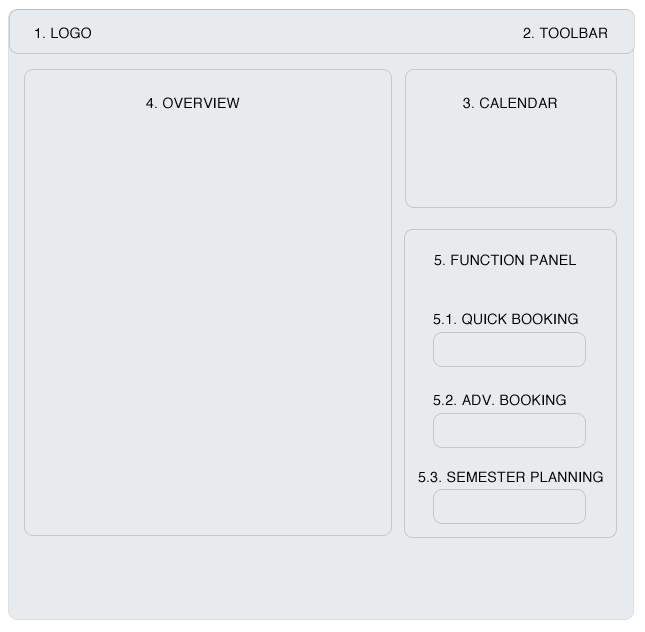
\includegraphics[width=0.6\textwidth]{images/wireframe1}
\end{center}
\caption{Wireframe for the frontpage}
\label{fig:wireframe_frontpage}
\end{figure}

\begin{itemize}
	\item \textbf{1. Logo}\\
	The logo for the application, which by convention should be located in the top left corner and link to the frontpage. \cite{steve}
	\item \textbf{2. Toolbar}\\
	A navigation toolbar. Should be used to login and logout, and for accessing the personal user account overview.
	\item \textbf{3. Calendar}\\
	An object used to navigate to a specific day in the future (or past).
	\item \textbf{4. Overview}\\
	The main overview, which should present a map of the university.
	\item \textbf{5. Function panel}\\
	A panel containing buttons used to enter the booking interface, or the semester planning.
\end{itemize}

\emph{We will refer to the different wireframe sections as (wire:section). For example, the advanced booking button is referred to as (wire:5.2).} 

\subsection{First round}
\subsubsection{Mockup}
\label{sub:first_mockup}
The first thing we wanted to test was the booking dialogue, as this was a major part of the user interaction. When the user selected a room on the map, the dialogue seen in figure \ref{fig:book_room_mockup} should appear in the function panel (wire:5)
 We wanted to give the user the impression that they never left the homepage, and to make sure no-one got lost in subscreens and menus.
\begin{figure}[htb]
\begin{center}
\leavevmode
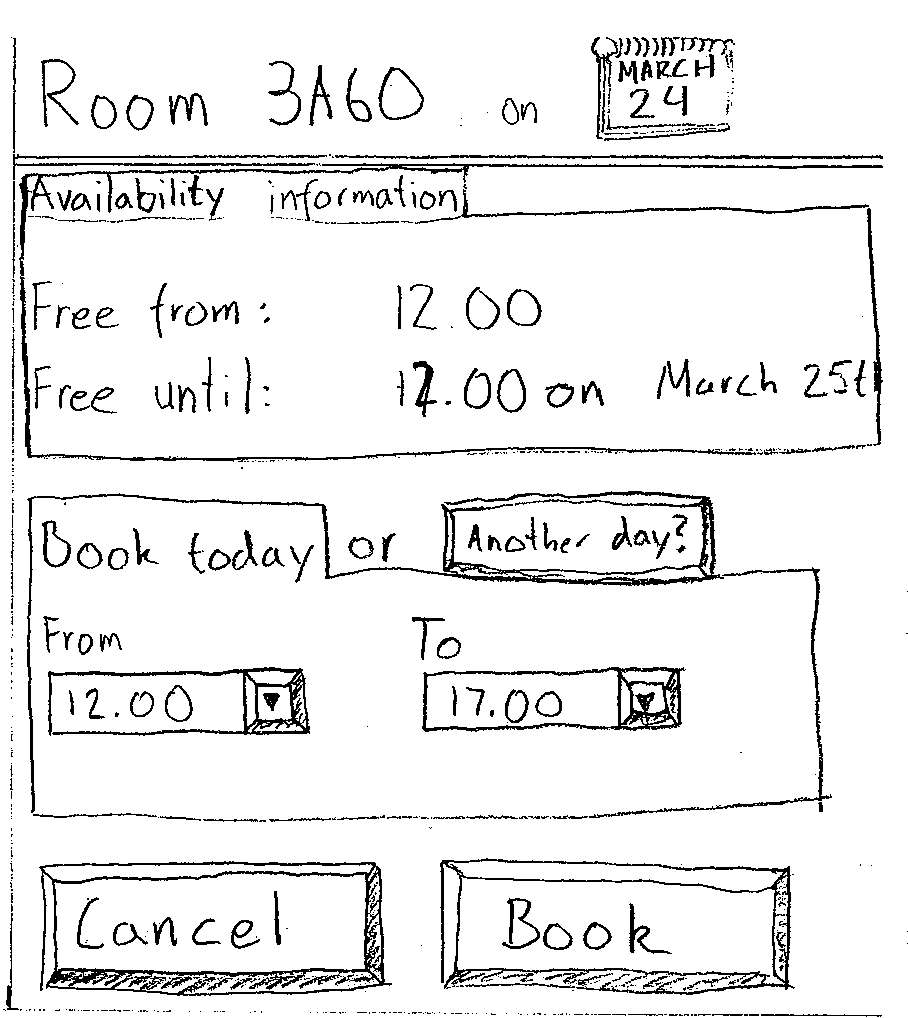
\includegraphics[width=0.6\textwidth]{images/bookRoomMockup}
\end{center}
\caption{First draft of the booking panel}
\label{fig:book_room_mockup}
\end{figure}

\subsubsection{Test}
\label{mock1:test}
In our first usability test, the users were to complete the following tasks:

\begin{enumerate}
	\item Find a random room
	\item Find a random room tomorrow
	\item Find a specific room
	\item Various variations of tasks involving finding rooms with specific requirements
\end{enumerate}

All the users had no problems completing task 1-3, but when the rooms needed to fulfil specific requirements, the  users felt overwhelmed by the amount of options, and did not spot the vital functions due to too much noise. This resultet in a task-failure for all test users. Also, our \emph{another day} button was often ignored. \\

What may come as a surprise, is that both users at some point or the other, tried to complete the simple tasks by using the advanced search button (wire:5.2) instead of e.g. using the map to select a room (wire:4). \\
\pagebreak


\subsection{Second round}
\subsubsection{Mockup}
\begin{figure}[htb]
\begin{center}
\leavevmode
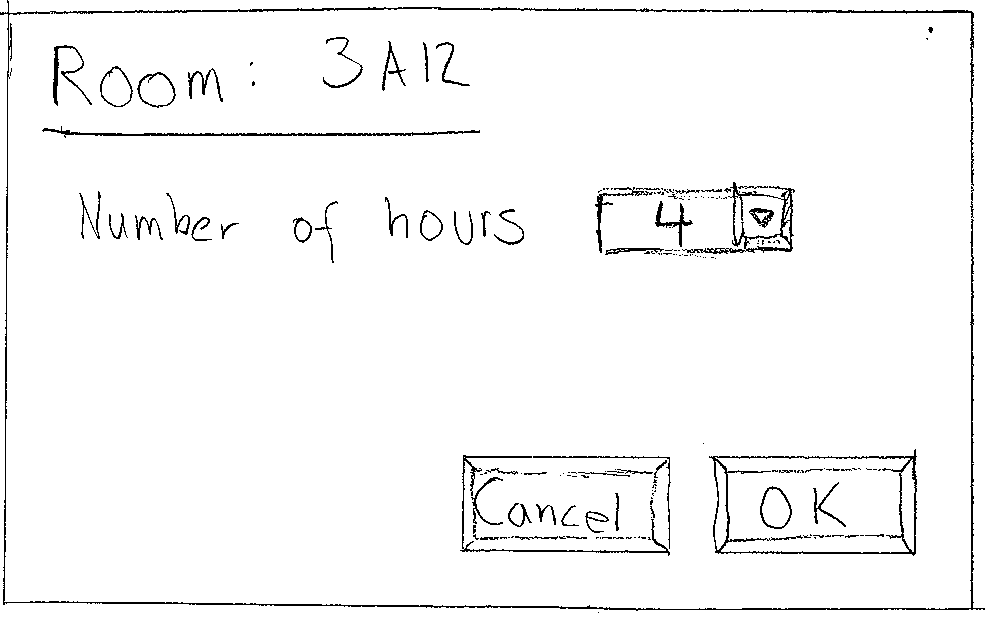
\includegraphics[width=0.8\textwidth]{images/bookRoomMockup2}
\end{center}
\caption{Second attempt at the simple booking. This time as a window overlaying the overview (wire:4)}
\label{fig:book_room_mockup2}
\end{figure}

Second time around, we tried making it as basic as possible to reduce the clutter, to make the users realize that this screen was for very simple tasks. We simply presented the user with a dialogue for selecting how many hours from now the room should be booked. This made all the test users pass the simple booking task, and it made them realize that the advanced search button(wire:5.2) should be used for tasks including specific room requirements. It did present another problem though: Now, no test users were able to figure out the availability of a room in the near future, as there was no button indicating this functionality when you had selected a room. The calendar (wire:3) was actually intended for this purpose, but this was not used by any of the users.\\

\subsubsection{test}
This round of testing was probably the one with the biggest impact on the final design. As shown on the test results from figure \ref{fig:results_day}, \emph{quick booking} was not thought of yet in the first round. Even though it created another problem of not providing the needed functional for getting a weekly overview, we discovered general satisfaction with the simplicity of the overlaying panel seen in figure \ref{fig:book_room_mockup2}. We wanted to keep this simplicity, while still making sure users could find a week overview of each room, which led to a very different third iteration.
\pagebreak

\subsection{Third round}
\subsubsection{Mockup}
\begin{figure}[htb]
\begin{center}
\leavevmode
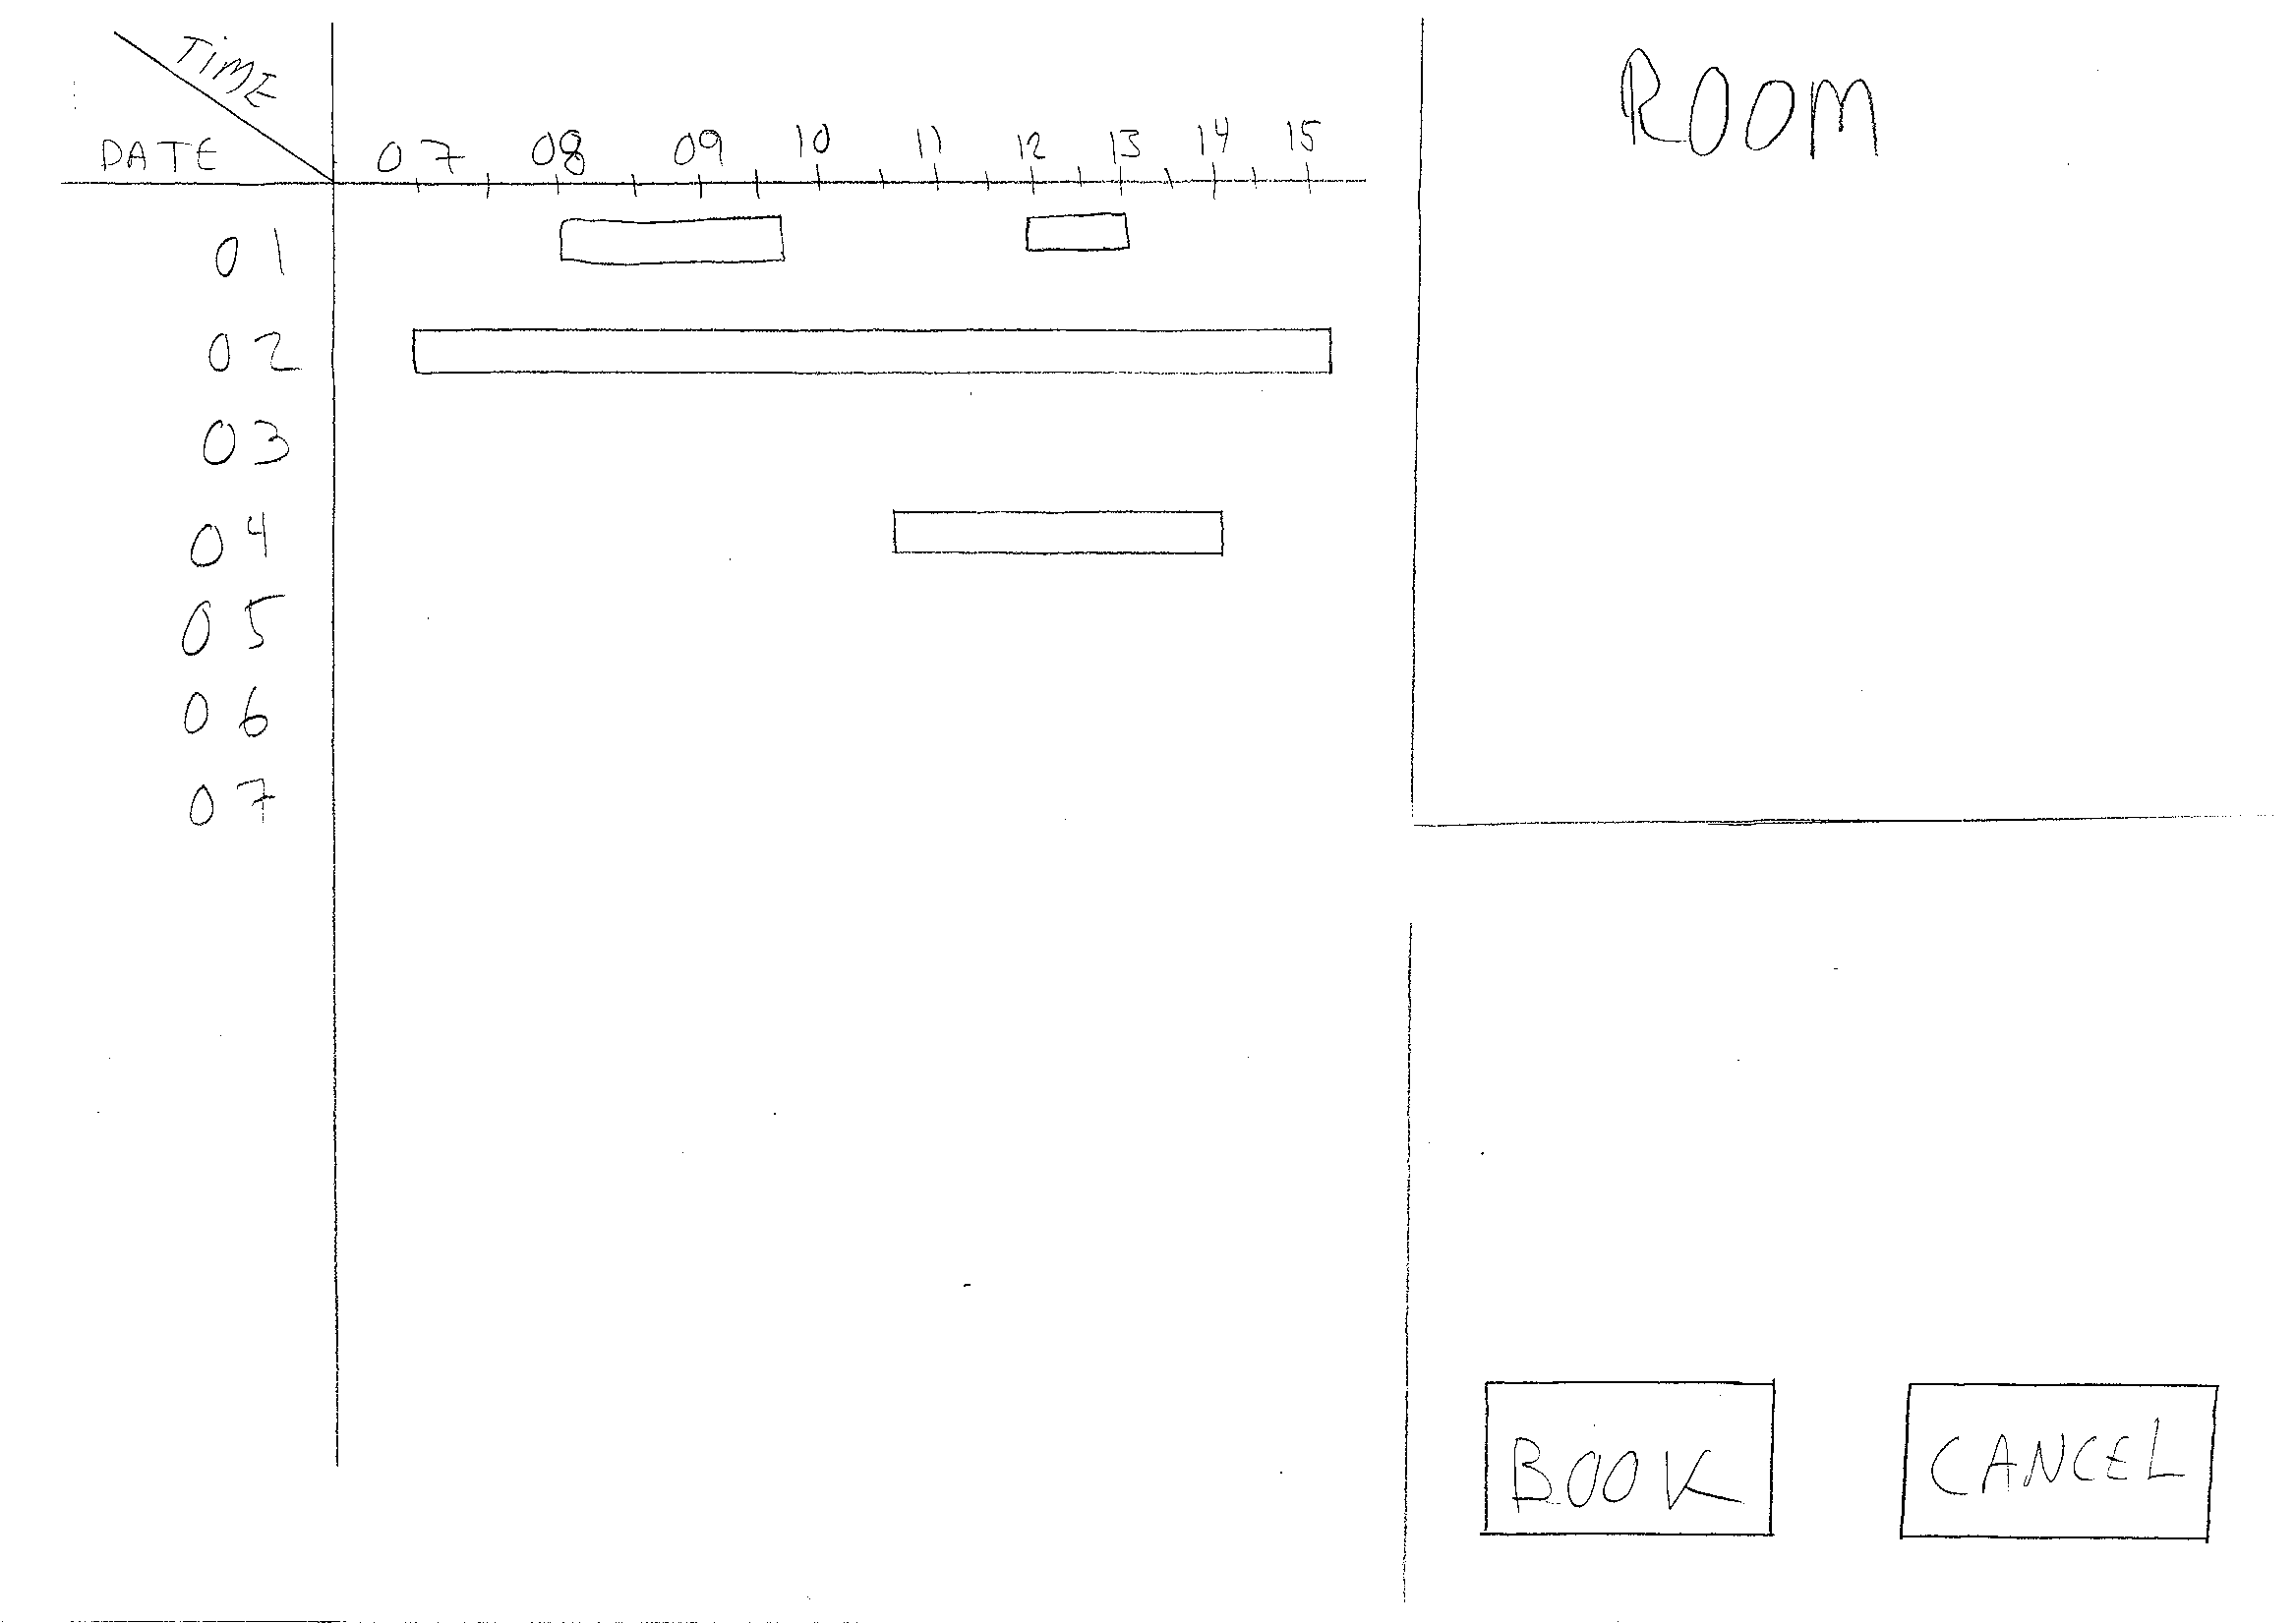
\includegraphics[width=0.8\textwidth]{images/weekMockup}
\end{center}
\caption{The mockup screen for a week overview on a specific room.}
\label{fig:week_mockup}
\end{figure}

In previous mockups, both users clicked on the specific room in an attempt to find the weekly overview.
In this iteration, we changed the mockup to do exactly this. When the users clicked on a room on the map (wire:4), the screen would change to the view in figure \ref{fig:week_mockup}.\\

As shown, we have decided to invert the x/y-axes as opposed to normal day-time overviews in eg. Outlook or Google Calendar. This is done because of the standard timeline being from left to right, and not top to bottom. We have simply added 7 timelines on top of each, as we thought it more intuitive when trying to get an overview. Our assumptions proved correct from every single test, as not a single user had a problem understanding the view immediately.\\

\subsubsection{Test}
All the test subjects used this overview effectively, when trying to book a room for a day not being the current. While the users passed the simple room booking tests in the second iteration, we did not test this again, but changed the function slightly due to new information gained through our domain research (see section \ref{xx}). The 'find me a room' button (wire:5.1) did not present the users with an option to choose the duration of the booking anymore, but simply booked the room for 4 hours. The user would then have the opportunity to extend the booking if necessary. Also, the room was now booked immediatly as the user clicked the button, to prevent problems with concurrent bookings, as discussed later in section \ref{xx}. Finally, we changed the label from 'Find me a room', to 'Quick Booking', to better reflect the actual functionality of the button.\\
Figure \ref{fig:quick_overlay} in the proposed design section shows the quick booking dialogue as presented to the user.


\pagebreak
\subsection{Final round}
\begin{figure}[htb]
\begin{center}
\leavevmode
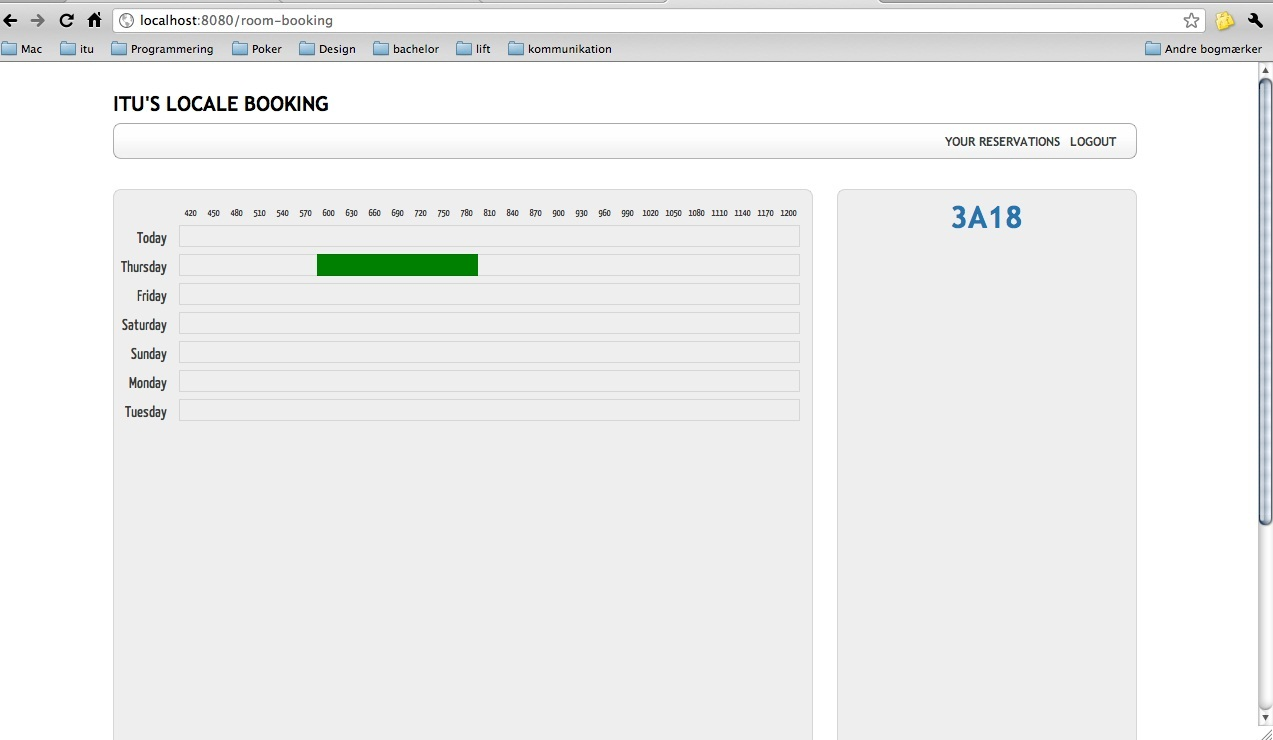
\includegraphics[width=1\textwidth]{images/weekFinal}
\end{center}
\caption{The finished screen for a week overview on a specific room, also used by Simple booking.}
\label{fig:week_final}
\end{figure}

The final design to book a room, as shown on figure \ref{fig:week_final}, grants an availability overview of 7 days, starting with the current day. Through our tests, we noted test subjects trying to drag the mouse to select, and others clicking for a start time followed by a click on end time, so we have chosen to allow for both.
To further assist the user in figuring out how it works, we have added highlighting of both the day and time when mouse is moved across the matrix.

The test results in figure \ref{fig:results_day} show a task failure for simple booking in third round, which was caused by him not discovering that the map was clickable, but once we intervened and directed him towards this view, he did succeed.

We have not conducted extensive tests for the final round, but simply performed sanity checks with previous test subjects, due to the reasonably small amount of changes between the rounds.


\pagebreak
\subsection{Proposed design}
\label{sec:proposed_design_dtd}
The process described above have naturally been repeated for each part of the system, resulting in our proposed design for the final interface.
Following is a description of all the screens that have been implemented, and their respective functions.

\subsubsection*{Front page}
\begin{figure}[htb]
\begin{center}
\leavevmode
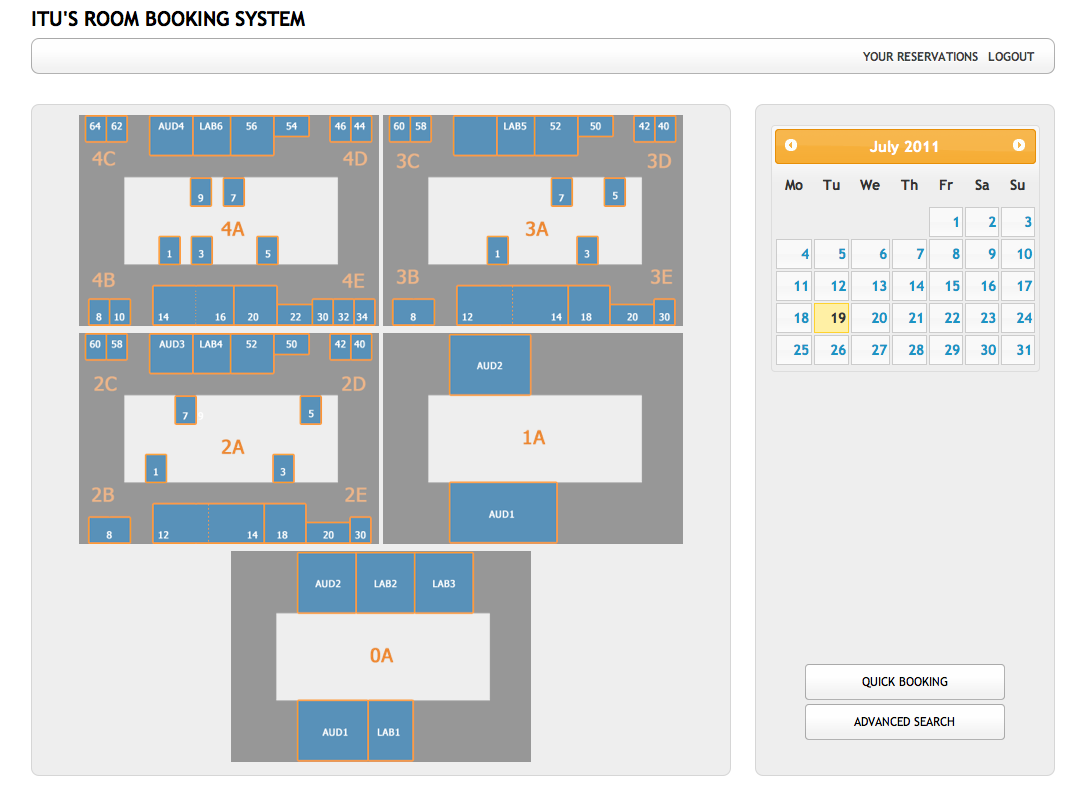
\includegraphics[width=1\textwidth]{images/frontpage}
\end{center}
\caption{The finished frontpage design}
\label{fig:frontpage}
\end{figure}
The frontpage shown on figure \ref{fig:frontpage} adheres a lot to the wireframe described above. 
We have made a couple of important decisions with the design. First off, we have decided to resize the rooms on the overview so they do not match the actual size of the rooms in reality. We have of course kept the location, and the approximate scale to adjecent rooms, but all the very small rooms have been enlarged to allow for easier selection.
Secondly, all offices, bathrooms, closets and kitchens have been left out. This is done to reduce clutter, and emphasize the rooms we are concerned with.

\pagebreak
\subsubsection*{Quick Booking}
\begin{figure}[htb]
\begin{center}
\leavevmode
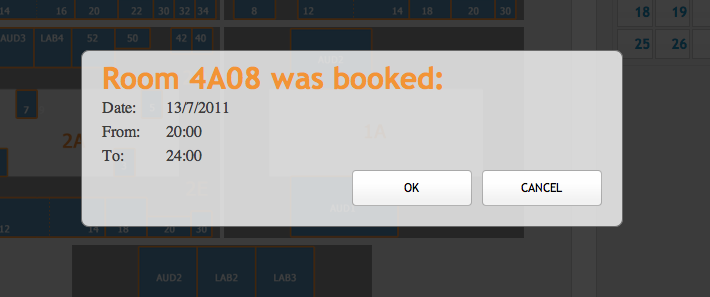
\includegraphics[width=1\textwidth]{images/quick_booking}
\end{center}
\caption{The overlay when quick booking is pressed}
\label{fig:quick_overlay}
\end{figure}
Shown on figure \ref{fig:quick_overlay} is the overlay appearing when the 'Quick Booking'-button is pressed.
It simply finds the smallest available room and books it for a default 4-hour span. The technicalities behind this function is described further in section \ref{XX}.

\pagebreak
\subsubsection*{Simple Booking}
\begin{figure}[htb]
\begin{center}
\leavevmode
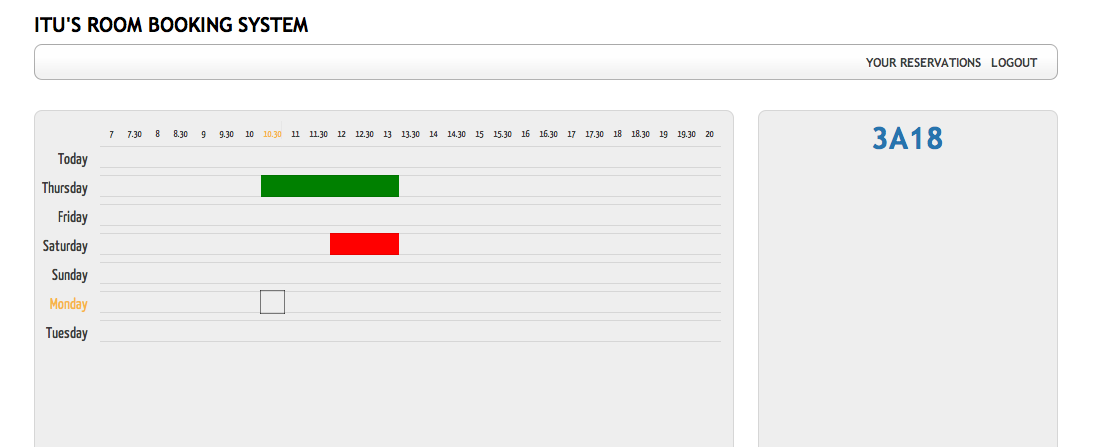
\includegraphics[width=1\textwidth]{images/simple_booking}
\end{center}
\caption{The overview and simple booking screen used when a specific room is clicked on the map}
\label{fig:simple_booking}
\end{figure}
When a specific room on the map overview is clicked, the screen displayed on figure \ref{fig:simple_booking} will be presented. The specifics of this part of the system has been discussed on in the example of the design process in section \ref{sec:design_process}.
It is worth noting that it only shows a 7-day overview, starting with today. We have considered to allow for scrolling back and forth in weeks, to allow the curious users to check bookings further in the future than a week.
We decided to not implement it in the prototype, as it would be an unnecesarry distraction for almost all situations this view would be used for.
Our tests revealed that users tend to utilize 'Advanced Search' for everything that was not immediately easy, and we concluded that if a booking needed to be made far in the future, that would be the function they used.

\pagebreak
\subsubsection*{Advanced Booking}
\begin{figure}[htb]
\begin{center}
\leavevmode
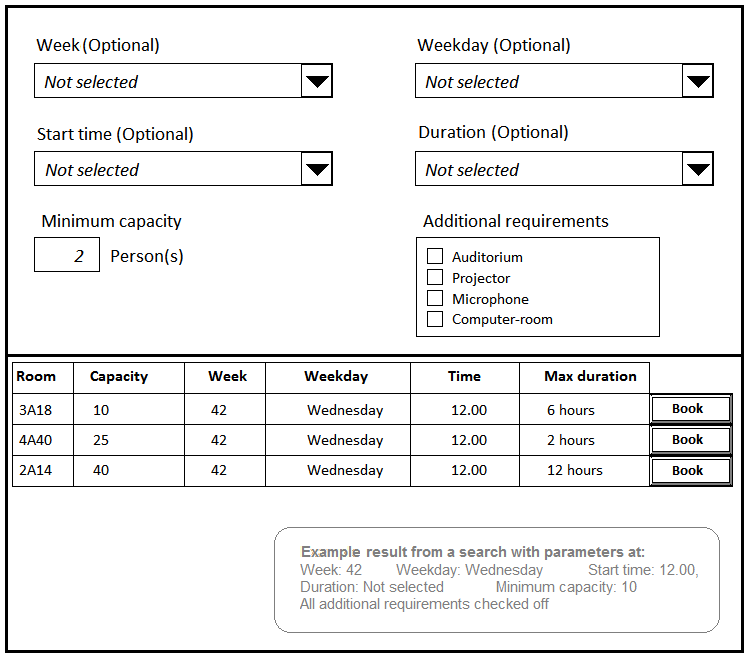
\includegraphics[width=1\textwidth]{images/advanced_mockup}
\end{center}
\caption{The design of the not-implemented advanced booking.}
\label{fig:advanced_mockup}
\end{figure}
The mockup on figure \ref{fig:advanced_mockup} shows the concept for our advanced booking screen. We have not made a search button, but instead allowed the result section to update dynamically for each parameter entered.
Note that the search result pane is filled with results from an example search, and does not correspond to the displayed default values in the form above.

The narrow design allows it to only overlay the map, and thus leave the calendar still visible. 
If a date is clicked on the calendar, the week number and day is filled into the search form. This functionality is not advertised by text, as it is not necesarry to succesfully use the system, and the text should be either very long, or run the risk of being confusing rather than helpful.\cite{steve}

\pagebreak
\subsubsection*{Your Reservations}
\begin{figure}[htb]
\begin{center}
\leavevmode
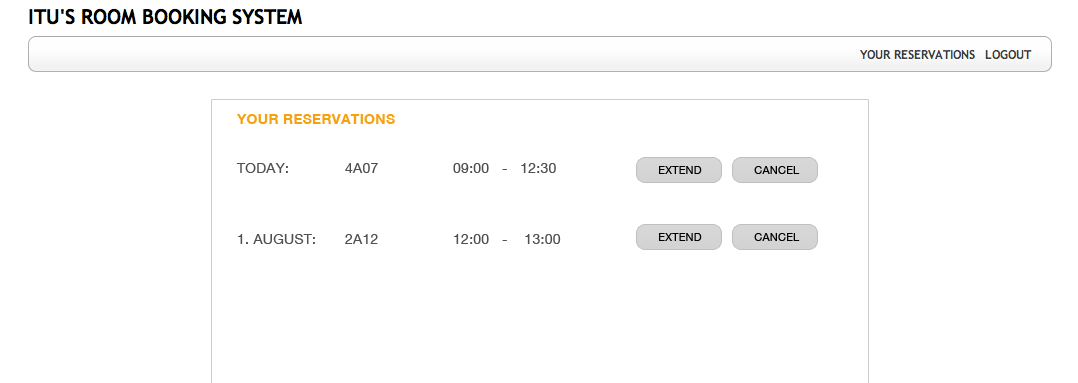
\includegraphics[width=1\textwidth]{images/reservations}
\end{center}
\caption{A users overview of ongoing/upcoming bookings}
\label{fig:reservations}
\end{figure}
The personal reservation screen, reached by the link in the top menu, is displayed on figure \ref{fig:reservations}. We have decided to omit past bookings from the view, as they would serve no real purpose other than increasing clutter for very active users.

\section{Semester planning}
\label{sec:semester_planning_ui}
\todo{fill this} %The key challenge for designing the semester planning user interface, is to find an optimal way to represent the data.

\subsection{Wireframe}
\label{subsec:wire_sem}
With our agile approach to designing the system, we have focused on getting testable mockups done as soon as possible. For most of the screens in the semester planning, this means drawing on a whiteboard where we can quickly add, remove and edit the screens until we have a satisfactory mockup, based on the data collected from interviews and analysis. However, for the screens which contains a lot of information, or requires a lot of user input, we have utilized the wireframe again to try and organize the data more systematic.

\begin{figure}[htb]
\begin{center}
\leavevmode
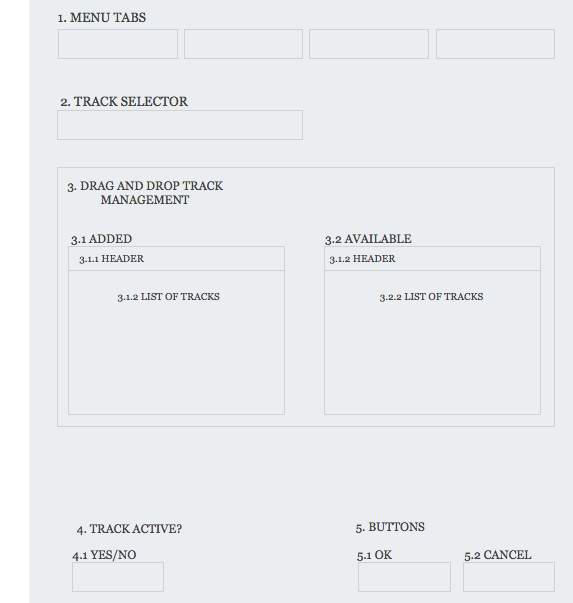
\includegraphics[width=0.6\textwidth]{images/wireframe_tracks}
\end{center}
\caption{Wireframe for the track management}
\label{fig:wireframe_tracks}
\end{figure}

Our first whiteboard mockups had track assignment done via the course management, where the user would add the tracks to a course as it was created. We quickly realized that by decentralizing the track management and handling it on a course to course basis, an important overview would be lost.

This lead us to take all things track related away from the course management, and add it to a wireframe, shown on figure \ref{fig:wireframe_tracks}. With a single view for all things track-related, confusion is less likely as users will not need to browse different screens, to gather all information the subject\cite{lauesen}.

The same view have been utilized for the teacher management, both out of convenience, and to reduce the amount of learning needed to succesfully use the system.


\subsection{Design phase}
\label{subsec:design_phase_sem}
\subsubsection{Limiting the test}
Our tests for the semester planning have not been as numourous as for the day to day booking, they have however been a lot more extensive in terms of time, tasks and discussions.
We interviewed the member of Study Administration who currently handles the semester planning, and tested our mockups with her aswell.

The advantages of having \emph{the} end-user available through the process are significant. It allows us to potentially leap over several iterations, as we can make the initial mockups a lot more detailed. Additionally, we can draw constant feedback and inspiration from a user with extensive domain-specific knowledge.
It is important to note that there are potential pitfalls connected with this aswell. By narrowing down our test users, we run the risk of hiding potential issues that our specific test subject solves with tacit knowledge.

\todo{forklar at dette er forskellen paa det vi siger (og citerer) i dtd booking om representable users}

Our justification for limiting the testing to our expert end-user is based on several things. First, due to the system being custom made for the ITU, the value of testing with a broader audience diminish due to lack of domain knowledge held by the actual end-user(s). Secondly, the system is being developed under time constraints, and with the diminishing value in mind, we deemed the trade-off to be reasonable. 

\subsubsection{Data views}
\begin{figure}[htb]
\begin{center}
\leavevmode
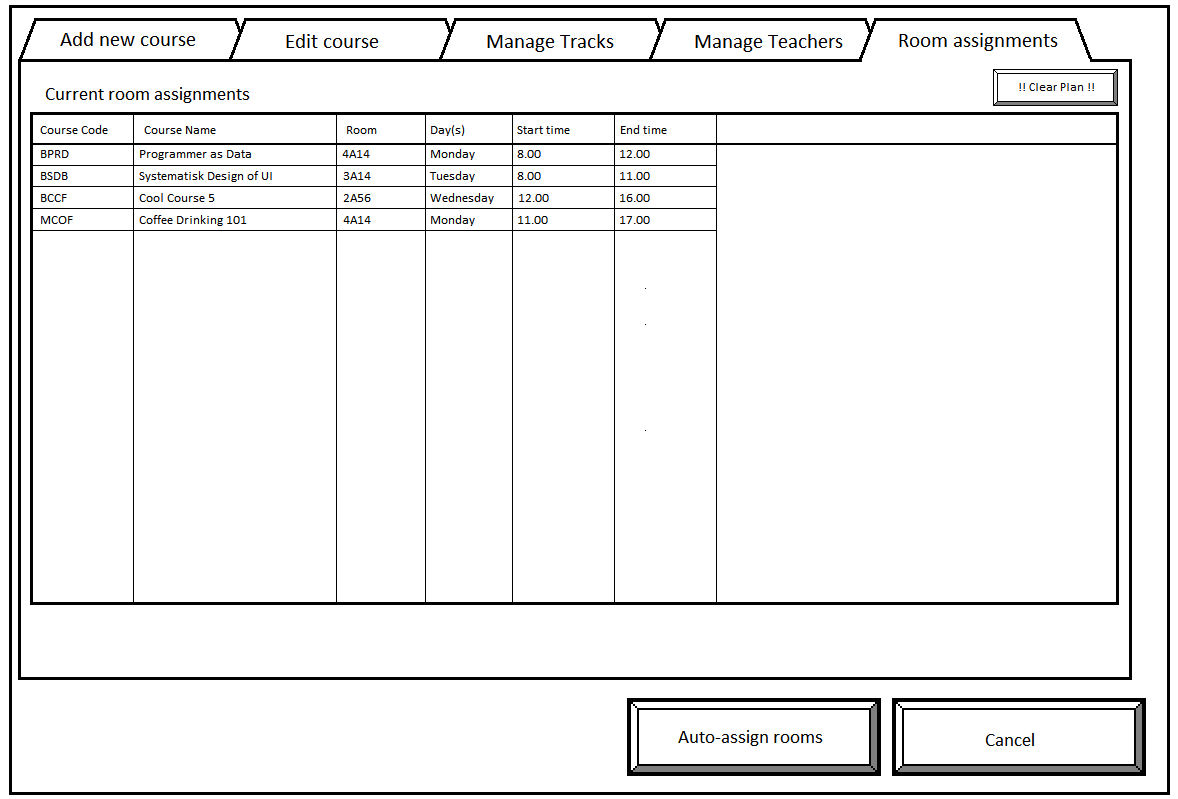
\includegraphics[width=0.8\textwidth]{images/sem1_room_assignments}
\end{center}
\caption{First version of the result screen from a succesful semester plan (with only 4 courses)}
\label{fig:sem1_room_ass}
\end{figure}

On figure \ref{fig:sem1_room_ass} is the first effort for the result screen. The idea was to conceal data which was not immidiately critical to the assignment, thus leaving more room for relevant data.
When this was put to the test, it was revealed that even though it was designed based on an interview, it was insufficient to our test subject; she wanted to see how each track was assigned.
Moving along, the list view remained in place, though expanded with additional sortable columns, but a new view was added to assist in the track overview.

\begin{figure}[htb]
\begin{center}
\leavevmode
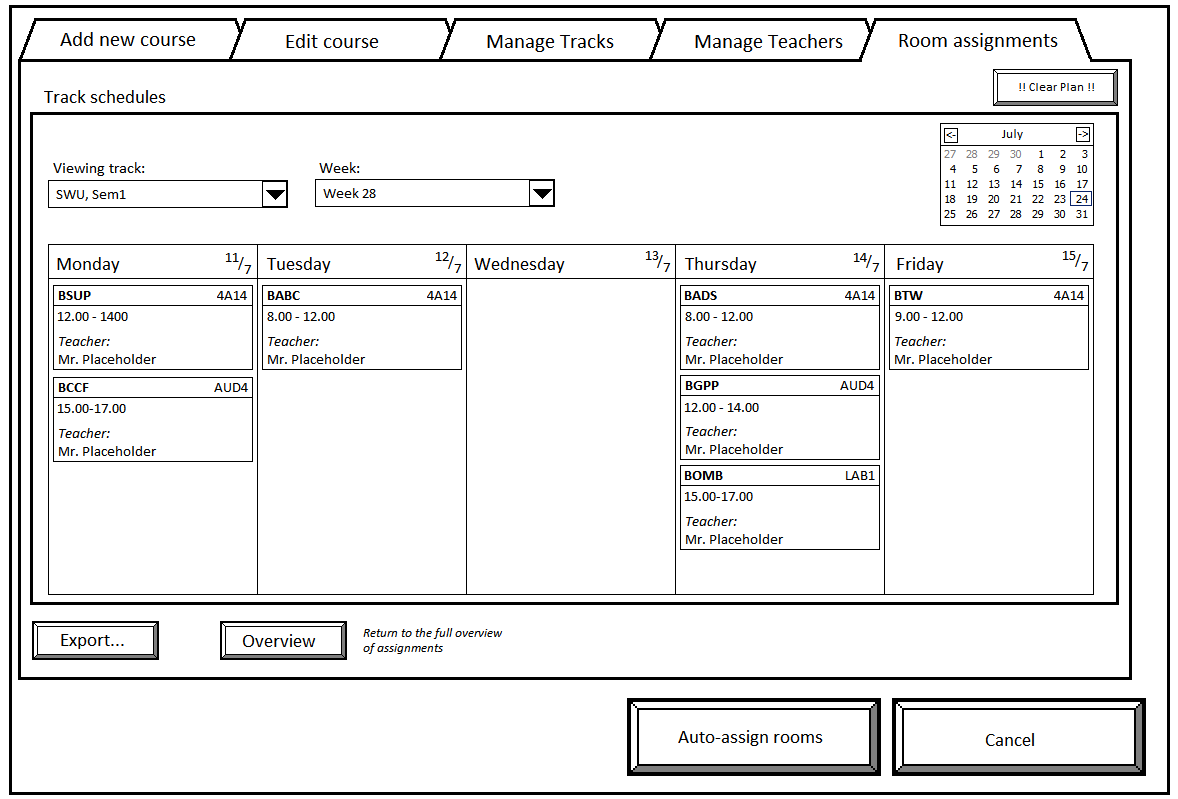
\includegraphics[width=0.8\textwidth]{images/sem2_room_sche}
\end{center}
\caption{The schedule overview added in second iteration}
\label{fig:sem2_room_sche}
\end{figure}

Figure \ref{fig:sem2_room_sche} shows an example schedule for a track.

\todo{maybe more, else fuck it}

\subsection{Proposed design}
\label{subsec:proposed_design_sem}

Following is a description of all the screens needed to complete a semester plan.

\subsubsection{Add course}
\begin{figure}[htb]
\begin{center}
\leavevmode
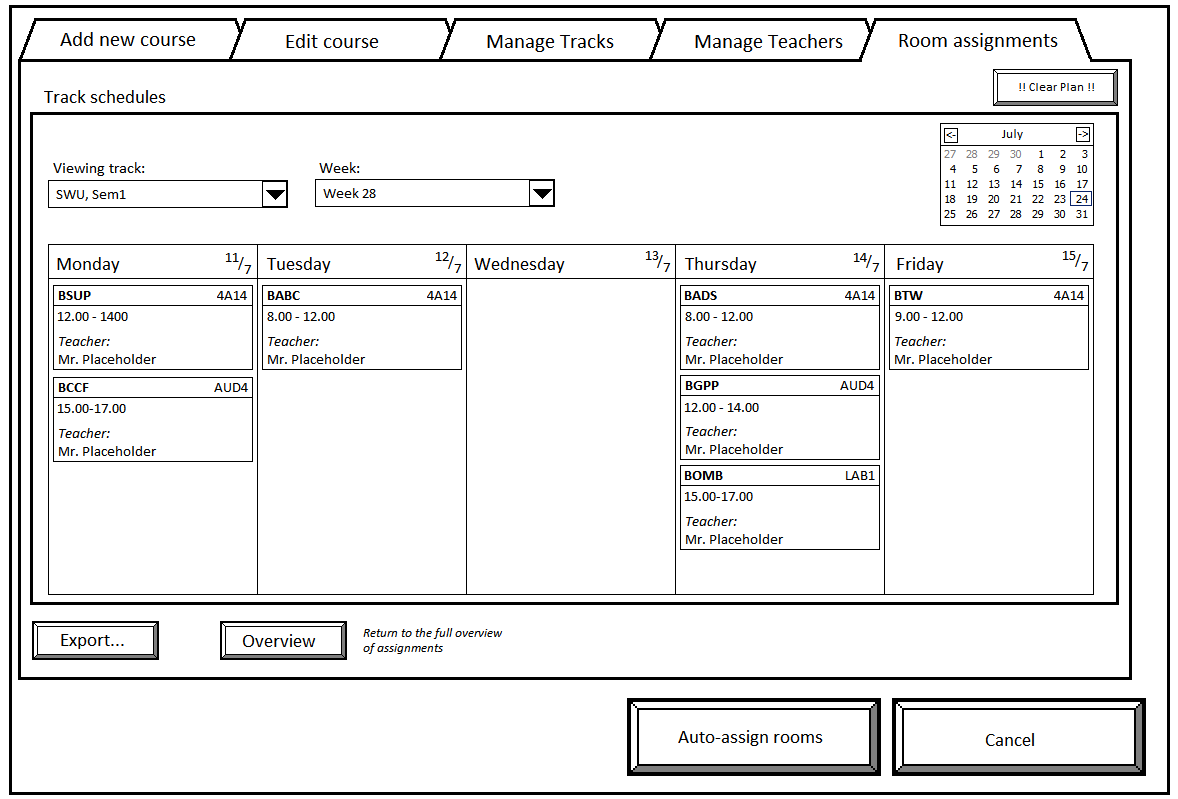
\includegraphics[width=0.8\textwidth]{images/sem2_room_sche}
\end{center}
\caption{The schedule overview added in second iteration}
\label{fig:sem2_room_sche}
\end{figure}





